\section{Introduction}
%% this is what I will do with my report. theory for basic understanding
%% then in turn methods and results.
Second sound is the propagation of heat in waves through superfluid.
Heat waves can be created with cyclic $I^2 R$ heating on a resistive coil,
and measured with an Allen Bradley carbon resistor.

The velocity will be measured in a cryogenic environment using resonance at a fixed
temperature with different harmonics for added accuracy, then the cryogenic environment
is allowed to heated up and the frequency of the
$n=1$ fundamental harmonic frequency is tracked.

This report the experiment is split into: cooling the apparatus and helium to a
superfluid and measuring the temperature for calibration when warming back up;
resonance of the the superfluid with $I^2 R$ heating for different harmonic
frequency inside of a resonance chamber in the
cryogenic environment, with which the velocity of the second sound is calculated;
and finally the fundamental frequency changing over temperature.

\subsection{History}
%% super-brief version of how superfluids came about and when and who.

\begin{figure*}[htbp]
\centering
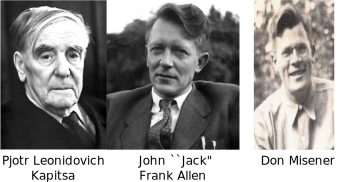
\includegraphics{pics/history.pdf}
\caption{ Physisics discovering Superfluidity in Helium in 1937. \label{fig:history}}
\end{figure*}

Don Misener (a graduate of University of Toronto) and
John F. Allen  from Winnipeg Canada\cite{disofsuper} (a graduate of University of Manitoba) %[2]
discovered the superfluid phase of matter in 1937 using liquid helium in the
Royal Society Mond Laboratory in Cambridge, with there work published in nature 141, 75 \cite{allenandmisenernature}. %[3]
Byt also in 1937 Pyotr Leonidovich Kapitsa (a.k.a. Peter Kapitza) 1894 - 1984 a Soviet
Russian Physicist released a paper Nature 141 74 in the same January 8th 1938 issue of Nature
journal as J F Allen and D Misener. 
Both of the studies demonstrated no viscosity below a `transition temperature’ of 2.18K.

It was 40 years before the Nobel Orgnization\cite{kapitsanobelprize} awarded half of that current years %[4]
Nobel Prize for Physics to P. Kapitsa for his `` basic inventions and discoveries in the area
of low-temperature physics''. The work from the Mond Laboratory did not get the
same recognition other than a single sentence in the Nobel Citation.
An interesting read on the
controversy is available on \url{www.physics.utoronto.ca/~griffin/PW\%20article\%20griffin.pdf}

%%comment of the discovery of second sound.

%[3] J. F. Allen and A. D. Misener, Nature 141, 75 (1937) \cite{allenandmisenernature}
%[4]http://nobelprize.org/nobel_prizes/physics/laureates/1978/kapitsa-bio.html \cite{kapitsanobelprize}
%JF Allen.                                    

%http://particle.physics.ucdavis.edu/bios/Allen.html 
 
%[2] "The Discovery of Superfluidity" by Russell J. Donnelly in Physics Today (July 1995) p. 30 \cite{disofsuper}

\subsection{Relavance}
Superfluids are a relatively new field, less than 80 years old. Interesting 
systems that have a superfluids behaviour are, for example, rarefied cold atomic gasses with 
both fermions and bosons, electrons in superconductors, and it is thought that 
neutron stars are thought be be a fermionic superfluid.


